\documentclass[11pt]{article}
\usepackage[margin=0.9in]{geometry}
\usepackage[T1]{fontenc}
\usepackage{lmodern,microtype,graphicx,booktabs,enumitem,tabularx,amsmath}
\usepackage[hidelinks]{hyperref}
\setlist{nosep,leftmargin=*}
\setlength{\parskip}{4pt}\setlength{\parindent}{0pt}
\usepackage{titlesec}
\titlespacing*{\section}{0pt}{9pt}{3pt}
\titleformat{\section}{\normalsize\bfseries}{\thesection.}{0.5em}{}
\titlespacing*{\subsection}{0pt}{5pt}{2pt}
\titleformat{\subsection}{\small\bfseries}{}{0em}{}
\renewcommand{\thesection}{\alph{section}}

\title{\vspace{-1.4cm}\textbf{Modeling Day to Day Physiological Recovery from Consumer Wearables}\\[2pt]
\large Technical Blueprint: A Recovery State Space Model for Mood on LifeSnaps\vspace{-0.2cm}}
\author{Maitrey Phatak \\ \small Applied Machine Learning II (EEE 6778) \quad Project Deliverable 1.2 \quad m.phatak@ufl.edu}
\date{\vspace{-0.7cm}}

\begin{document}
\maketitle

\section{Problem Context and Project Summary}
Consumer wearables record sleep, heart rate, heart rate variability (HRV), and activity every day, yet models linking these signals to mood treat each day as an independent sample, or model sleep only within a single night. Physiology accumulates: sleep loss and exertion lower recovery for several days. This project builds a state space model in which a latent physiological recovery state evolves daily, driven by sleep and activity and observed through resting heart rate and HRV, and tests two claims on the LifeSnaps dataset \cite{lifesnaps}: (1) the latent state behaves like physiological recovery, and (2) coupling that state to mood, estimated per person, improves forecasts of self reported mood and relates to emotional stability. The deliverable is a reproducible modeling pipeline and an interactive explorer that shows each person's recovery trajectory, mood forecast, and how closely their mood tracks their physiology.

\subsection{Response to Deliverable 1.1 feedback}
\begin{tabularx}{\linewidth}{@{}p{0.33\linewidth}X@{}}
\toprule
Feedback item & Status \\ \midrule
Linear state space model first & \textbf{Done.} Stage 1 linear Gaussian model is fitted and evaluated (Section c); all later stages build on it. \\
4 months vs 8 weeks & \textbf{Reconciled from the data.} Median Fitbit span is 67 days and median mood reporting window is 57 days (about 8 weeks) per person; collection as a whole spans Apr 2021 to Jan 2022 across two cohorts. \\
Count days with mood labels & \textbf{Counted.} 63 of 71 people report mood; 2{,}290 labeled days; 48 people have $\geq$14 labeled days (analysis cohort). \\
Latent responds to short nights & \textbf{Tested.} Over 346 short nights the state drops and recovers over about 5 days (Figure 2). \\
Gains after disruptions & \textbf{Tested.} No gain specific to disruption days for the pooled model; motivates per person coupling (Section e). \\
New people in leave one subject out & \textbf{Decided.} Report both population parameters only and parameters inferred from a new person's first 7 days. \\
Drop the Transformer first & \textbf{Done.} Transformer removed; LSTM kept as the deep sequence baseline. \\
Baseline in week one & \textbf{Done.} Carry forward: balanced accuracy 0.361 on the test period (chance 0.143). \\
\bottomrule
\end{tabularx}

\textbf{Contribution statement.} \emph{A state space model with a latent physiological recovery state, driven by sleep and activity and observed through resting heart rate and HRV, reproduces multi day recovery after short nights; per person coupling of that state to mood tests whether mood forecasts improve and whether people differ in how closely their mood tracks their physiology.}

\section{Dataset}
\textbf{Source and access.} LifeSnaps version 4 on Zenodo (DOI 10.5281/zenodo.7229547), CC BY 4.0, a single 615 MB archive. The project uses the provided CSVs: daily Fitbit and mood indicators (2.1 MB, 7{,}410 rows), hourly Fitbit and individual mood reports (21.1 MB, 159{,}508 rows), and the scored IPIP personality survey (50 people). The 9.7 GB MongoDB dump is not needed. Data type: multivariate tabular time series plus categorical self reports. The CSVs are committed in \texttt{data/raw} with attribution, as the license permits.

\textbf{Participants and labels.} 71 participants in two cohorts (46 starting April to June 2021, 25 starting October to November 2021). Each mood report selects one of seven categories (alert, happy, neutral, rested/relaxed, sad, tense/anxious, tired). The analysis cohort is the 48 people with at least 14 mood labeled days: 4{,}912 reports over 2{,}218 labeled days, a median of 93 reports per person. Report shares: rested/relaxed 23.5\%, tired 22.5\%, neutral 16.4\%, happy 15.7\%, tense/anxious 12.1\%, alert 6.9\%, sad 2.9\%. Mood varies by time of day (tense/anxious is 16\% of morning and 7\% of evening reports), so time of day enters every model.

\textbf{Signal coverage on mood labeled days.} Steps 91\%, resting heart rate 87\%, sleep 78\%, HRV (RMSSD) 51\% (31 of 48 people). Core inputs are steps, resting heart rate, and sleep; HRV is used where present.

\textbf{Preprocessing challenges.}
\begin{itemize}
\item \emph{Date alignment.} Fitbit assigns sleep to the date the sleep ended \cite{fitbitapi}; LifeSnaps preprocessing uses this convention for sleep and temperature, and 99.5\% of HRV dates coincide with sleep dates. Night signals are therefore paired with the same day's reports (previous night for reports before 6 am), while daily totals (steps, resting heart rate) are lagged one day to prevent leakage.
\item \emph{Missingness.} Calendar day coverage is 51 to 62\% for core signals. The state space model skips updates on missing observations; missing inputs are set to the person mean with an observed flag.
\item \emph{Implausible values.} RMSSD values of zero are set to missing.
\item \emph{Scale differences.} Signals are z scored within each person, so dynamics reflect deviations from each person's own baseline.
\end{itemize}

\textbf{Ethical and privacy considerations.} Participants consented to open release, and the data are anonymized under GDPR guidelines \cite{lifesnaps}. The project does not attempt re identification and reports only aggregate or pseudonymous results. The trait measure is Big Five emotional stability, since LifeSnaps STAI is the state version.

\section{Planned Architecture}
\begin{figure}[h]\centering
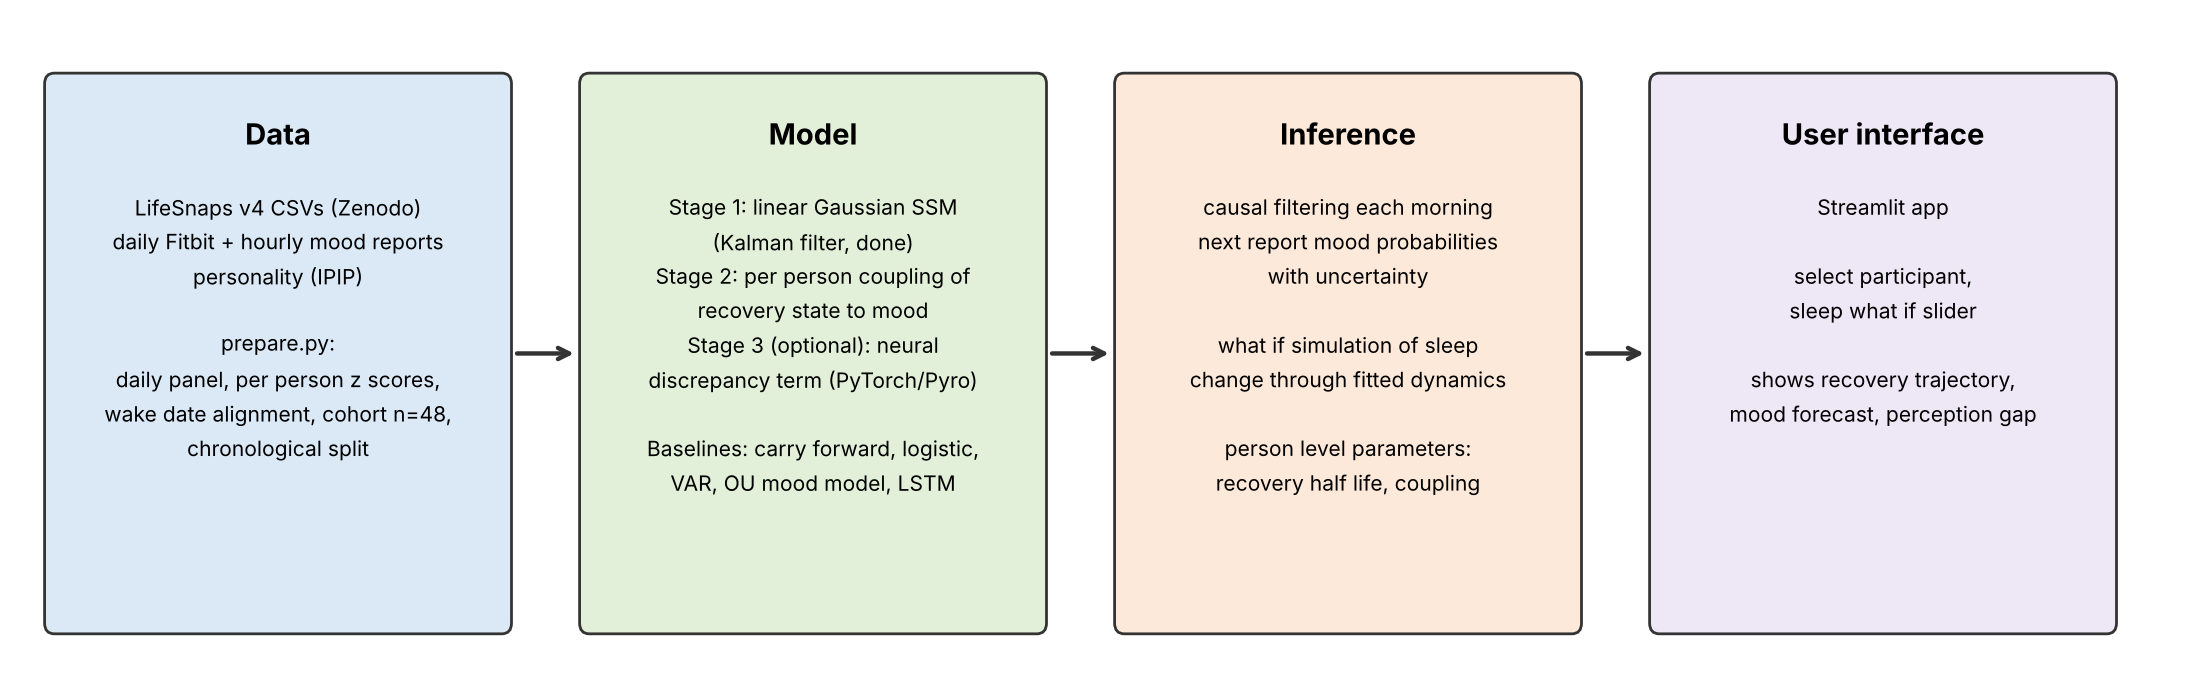
\includegraphics[width=\linewidth]{architecture.png}
\vspace{-14pt}\caption{\small Data flow from LifeSnaps CSVs to the interactive explorer.}
\end{figure}

\textbf{Stage 1 (completed): linear Gaussian state space model.} Latent $x_t$ is recovery on the morning of day $t$:
$x_t=\phi x_{t-1}+b_1\,\text{sleep}_t+b_2\,\text{efficiency}_t+b_3\,\text{steps}_{t-1}+w_t$, observed through HRV ($\text{rmssd}_t=c\,x_t+v_t$) and resting heart rate (loading fixed at $-1$ for scale). Parameters are fitted by maximum likelihood on training days with a causal Kalman filter, pooled across people. Fitted values: persistence $\phi=0.874$ (half life 5.1 days), sleep $+0.064$, efficiency $+0.032$, previous day steps $-0.076$, HRV loading $+0.48$. All signs are physiologically sensible. The resting heart rate noise reached its lower bound (0.1), indicating the state leans heavily on resting heart rate; Stage 2 addresses this with per person observation noise.

\begin{figure}[h]\centering
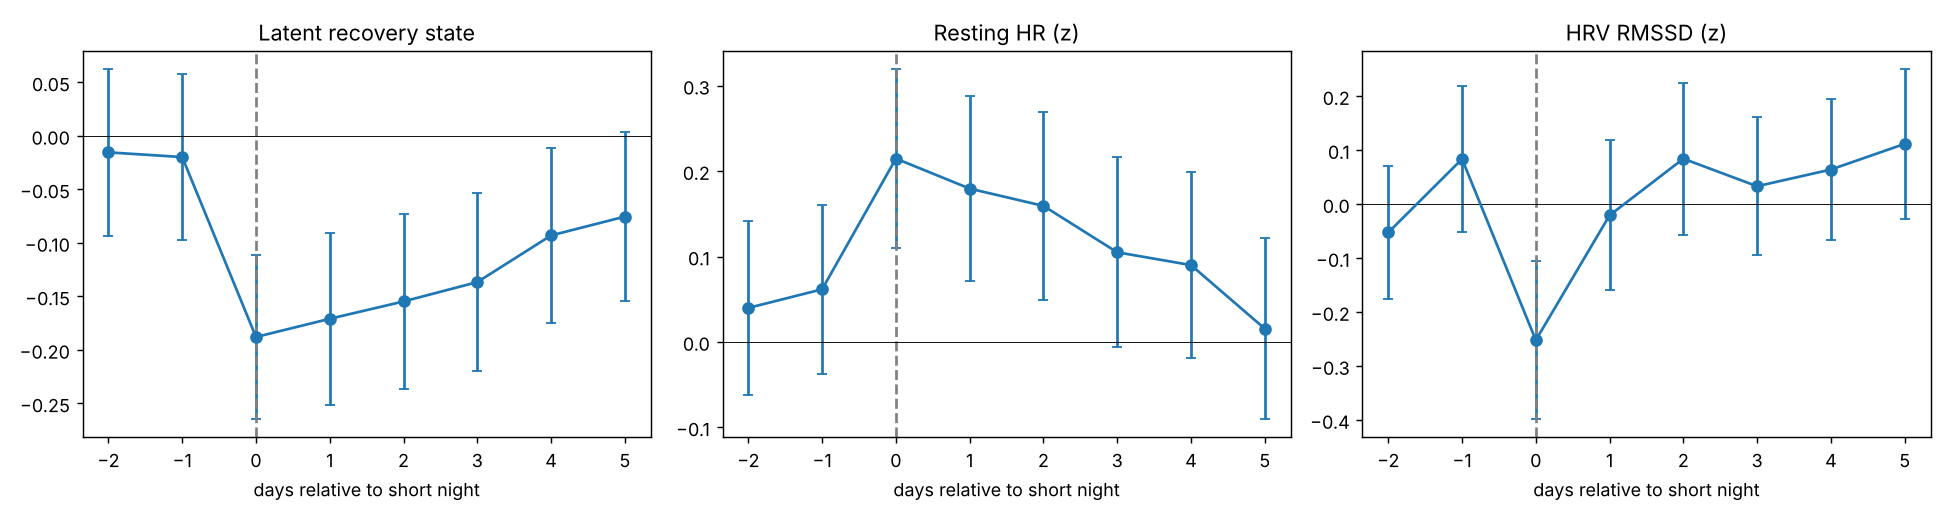
\includegraphics[width=0.95\linewidth]{event_locked_short_night.png}
\vspace{-8pt}\caption{\small Mean ($\pm$95\% CI) around 346 short nights (sleep more than 1 SD below the person's mean). The latent state drops and recovers over about 5 days; resting heart rate stays elevated for about 3 days; HRV drops for one night. The drop at day 0 is partly built in because sleep is an input; the multi day persistence comes from the learned dynamics.}
\end{figure}

\textbf{Mood model.} Each report's category is predicted from time of day, the previous report, and the filtered morning recovery state (multinomial logistic link). Evaluation uses each person's first 70\% of labeled days for training and the last 30\% for testing (1{,}354 test reports), with participant bootstrap confidence intervals.

\begin{center}\small
\begin{tabular}{@{}lccc@{}}
\toprule
Model (test period) & Balanced accuracy & Macro F1 & Log loss \\ \midrule
Carry forward (previous report) & 0.361 & 0.360 & -- \\
Time of day + previous mood & 0.374 & 0.334 & 1.730 \\
\quad + last night and previous day physiology & 0.348 & 0.313 & 1.734 \\
\quad + 5 day moving averages (accumulation control) & 0.360 & 0.320 & 1.745 \\
\quad + Stage 1 recovery state & 0.377 & 0.333 & 1.729 \\
\bottomrule
\end{tabular}
\end{center}
The recovery state is the best physiology variant and beats the moving average control, but its gain over time of day plus previous mood is not reliable (difference $+0.004$, 95\% CI $-0.012$ to $+0.023$).

\textbf{Planned stages and frameworks.}
\begin{itemize}
\item \emph{Stage 2: per person coupling.} Hierarchical model with a person specific coupling between recovery and each mood, and per person persistence and noise, sharing a population prior (Pyro, variational inference). Tests: forecast gain, variation in coupling across people beyond noise, and association with emotional stability controlling for mood mean, mood variability, and mood inertia.
\item \emph{Baselines to add:} vector autoregression (lagged sleep and mood), an Ornstein Uhlenbeck latent mood model (mood inertia without physiology), and an LSTM (PyTorch). The Transformer is dropped.
\item \emph{Stage 3 (optional):} a small neural network added to the transition as a discrepancy term, keeping the physiological structure.
\item \emph{Interface role:} Streamlit app that reads saved model outputs (filtered states, parameters, forecasts) and runs what if simulations through the fitted dynamics; it does not retrain models.
\end{itemize}

\section{User Interface Plan}
\textbf{Input.} The user selects a participant and date range, toggles HRV and mood report layers, and moves a what if slider that changes last night's sleep by up to two hours. A planned extension accepts an uploaded CSV in the same format.

\textbf{Output.} (1) The recovery trajectory with its 95\% band, overlaid on sleep, resting heart rate, and shaded disruption days; (2) next day mood probabilities by time of day, with what if bars beside the current forecast; (3) a perception gap panel showing the person's coupling strength, recovery half life, and a plain language explanation.

\textbf{Value.} The latent state is otherwise invisible. Plotting it beside raw signals lets a reviewer check whether it behaves like recovery, the what if slider exposes the model's counterfactual behavior directly, and showing uncertainty prevents overconfidence in single forecasts.
\begin{figure}[h]\centering
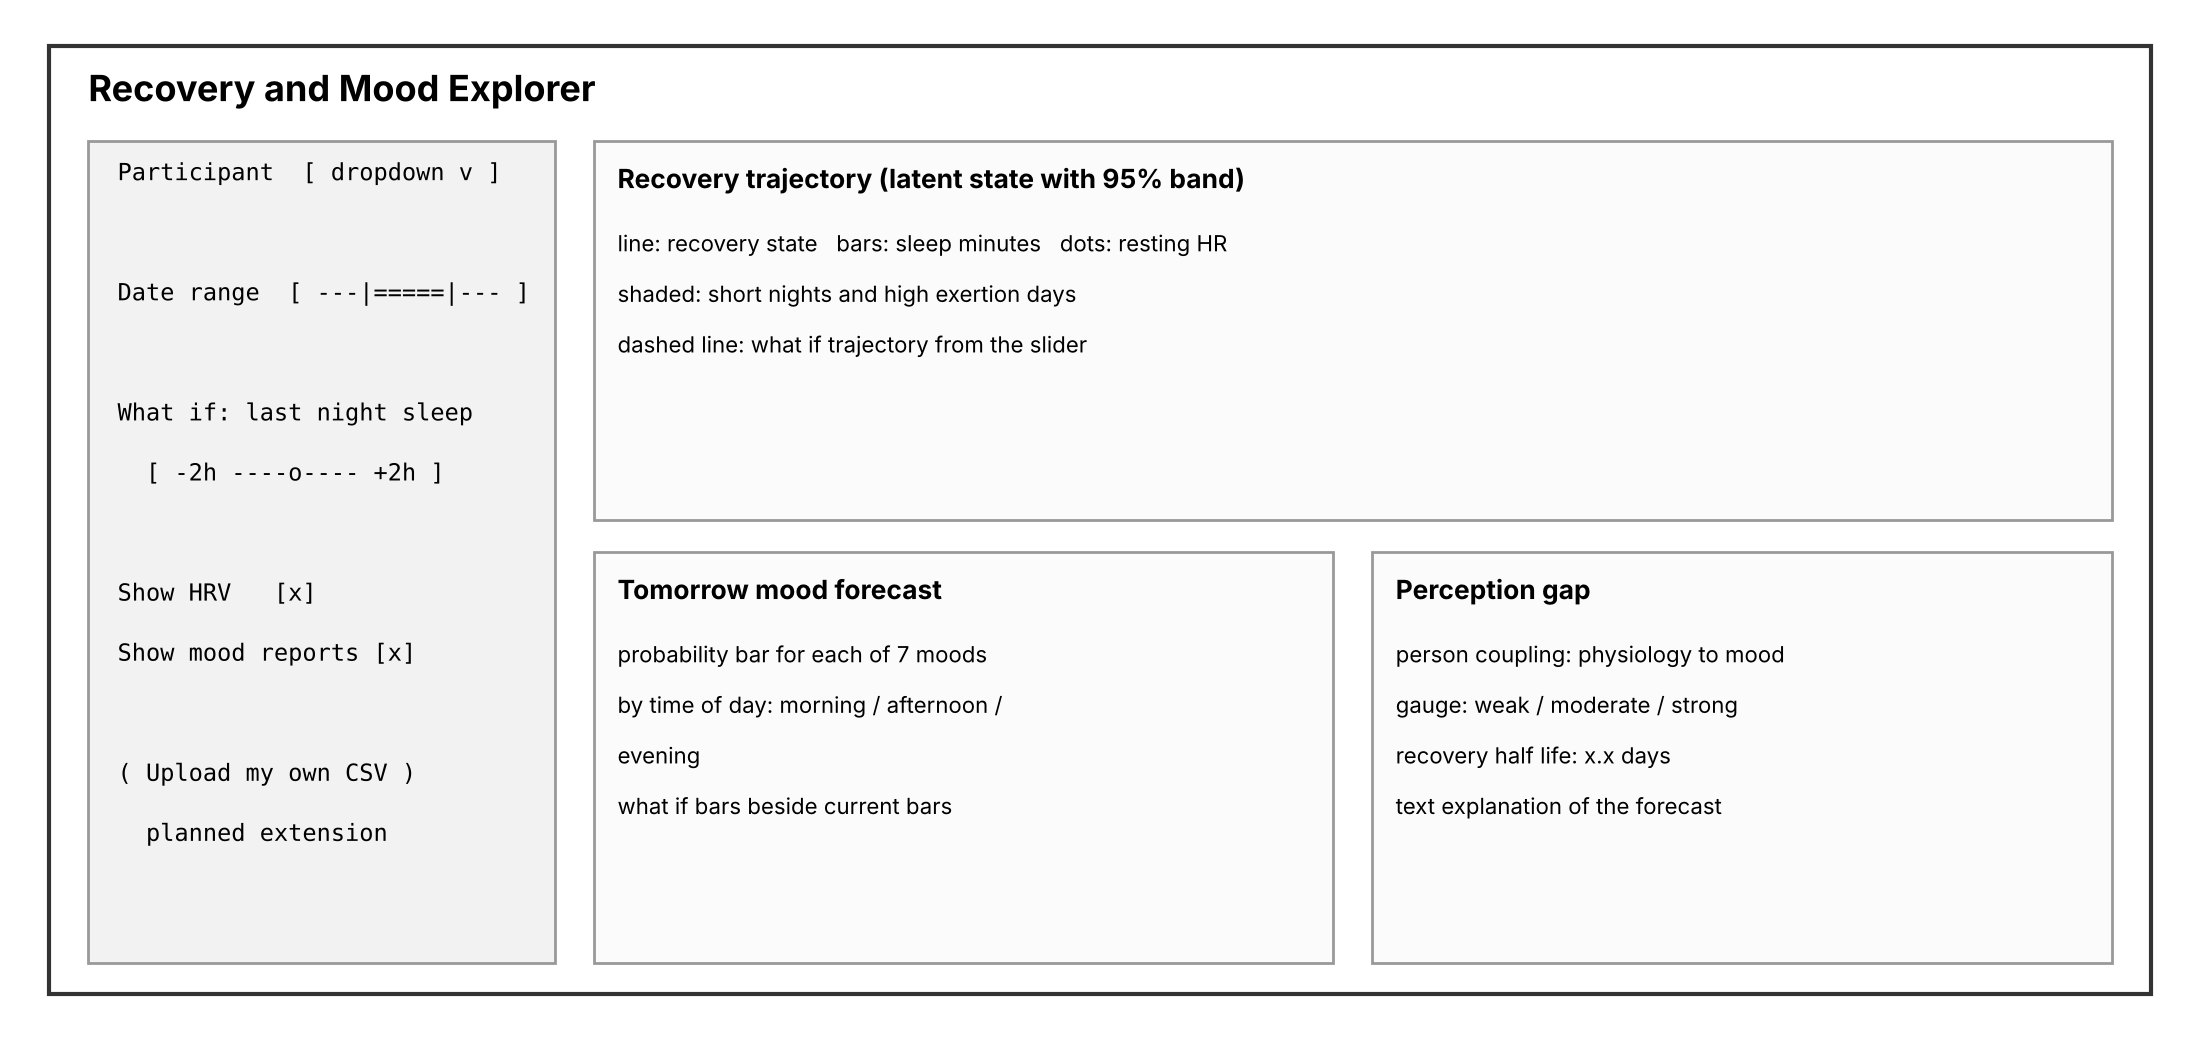
\includegraphics[width=0.92\linewidth]{wireframe.png}
\vspace{-8pt}\caption{\small Wireframe of the Streamlit explorer.}
\end{figure}

\section{Innovation and Anticipated Challenges}
\textbf{Innovation.} Deep state space models and sequence models for wearable mood already exist, so the contribution is not the model class. Prior LifeSnaps work classifies mood or stress from daily features or models sleep within a single night; psychology models mood as a latent process with inertia but without physiology. This project (1) builds the transition from established physiology (sleep restores, exertion loads, recovery decays) so the latent state has a defined meaning, (2) validates that meaning with tests a black box cannot pass (short night response, recovery half life against resting heart rate), and (3) estimates per person coupling between physiological recovery and felt mood, turning the known mismatch between wearable metrics and how people feel into a measured parameter.

\textbf{Risks and mitigation.}
\begin{enumerate}
\item \emph{Physiology may add little to mood forecasts.} Stage 1 already shows no reliable pooled gain. \emph{Mitigation:} the project reports this honestly and tests per person coupling; the recovery validation and the coupling distribution remain results even if forecast gains stay small.
\item \emph{Sparse labels and short sequences.} About 8 weeks per person with patchy reports. \emph{Mitigation:} hierarchical priors share strength across people, the latent dimension stays at one or two, and the model learns dynamics from all wearable days, not only labeled days.
\item \emph{Identifiability and training instability.} The latent state can collapse onto one signal, and variational training can be unstable. \emph{Mitigation:} noise floors and fixed loadings, initialization from Stage 1 estimates, and a synthetic data check that the model recovers known coupling and persistence values.
\end{enumerate}

\section{Implementation Timeline}
\begin{center}\small
\begin{tabularx}{\linewidth}{@{}p{2.3cm}Xp{4.6cm}@{}}
\toprule
Week & Focus & Expected outcome \\ \midrule
Nov 9 to 15 & Data audit, alignment, baselines, Stage 1 linear model, short night test & Completed: repository, setup notebook, Stage 1 results \\
Nov 16 to 22 & Stage 2 per person coupling; VAR, OU, LSTM baselines; synthetic recovery check & Stage 2 trained end to end; full baseline table \\
Nov 23 to 29 & Leave one subject out (both settings), emotional stability analysis, ablations; Streamlit prototype on saved outputs & Generalization and trait results; interface running \\
Nov 30 to Dec 6 & Optional neural discrepancy term; interpretability figures; interface refinement and demo & Stable interactive demo; final figures \\
Dec 7 to 9 & Final report and presentation & Completed project, presentation ready \\
\bottomrule
\end{tabularx}
\end{center}

\section{Responsible AI Reflection}
\textbf{Fairness.} LifeSnaps comes from four European countries and overrepresents young adults with normal BMI \cite{bias}, and the cohort is limited to people who reported mood regularly, so results may not transfer to older, clinical, or less engaged users. Results will be broken down by gender and cohort where sample sizes allow. \textbf{Transparency.} The model is interpretable by design, every forecast is shown with uncertainty, and the null pooled result is reported rather than hidden. \textbf{Misuse.} The tool is a research explorer, not a diagnostic device; mood forecasts are probabilistic and must not drive clinical decisions. \textbf{Privacy.} Only anonymized open data are used, and no attempt is made to link records to individuals. \textbf{Environmental cost.} All models are small and train on a CPU in minutes, so compute and energy use are minimal.

\vspace{-4pt}
\renewcommand{\refname}{\normalsize References}
\begin{thebibliography}{9}\small\setlength{\itemsep}{0pt}
\bibitem{lifesnaps} S. Yfantidou et al., ``LifeSnaps, a 4-month multi-modal dataset capturing unobtrusive snapshots of our lives in the wild,'' \emph{Scientific Data}, vol. 9, 663, 2022.
\bibitem{fitbitapi} Fitbit Web API Reference, ``Get Sleep Log by Date,'' dev.fitbit.com (dateOfSleep is the date the sleep log ended).
\bibitem{bias} S. Yfantidou et al., ``Uncovering the Hidden Biases in Personal Informatics,'' ACM, 2025.
\end{thebibliography}
\end{document}
